\section{Diagramme und Darstellungsweisen}
\subsection{Phasenverschiebung und $\mathbb{C}$-Ebene}
Die Phasenverschiebung des Frequenzspektrums ist bei der physikalischen Betrachtung nur in den wenigsten Fällen von Bedeutung. Der Hauptaugenmerk liegt auf der Verteilung der Amplituden.
Durch geschickte Verschiebung kann das Spektrum auch so verändert werden, dass das Signal y-achsensymmetrisch oder punktsymmerisch zum Ursprung ist. In diesen Fällen besteht das Frequenzspektrum nur aus den Orthonormalbasen, die diese Eigenschaften teilen.

Deshalb behilft man sich für eine zweidimensionale Darstellung entweder mit zweifarbigen Diagrammen für $Re(\hat{f}(\omega))$ und $Im(\hat{f}(\omega))$ oder es wird nur der Betrag der Amplitude $$ | \hat{f}(\omega) | = \sqrt{ Re(\hat{f}(\omega))^2 + Im(\hat{f}(\omega))^2 } $$ aufgetragen.

\subsection{Fast-Fourier-Transform}
Als Integraltransformation ist die Fouriertransformation universell einsetzbar, jedoch nur für wenige, kontinuiertliche Funktionen analytisch berechenbar. Da in der technischen Anwendung hauptsächlich diskrete Signale analysiert werden sollen, die zeitnah benötigt werden, behilft man sich einer anderen Technik.

Die diskrete Fouriertransformation (DFT) würde numerisch den Flächeninhalt für jede Oberschwingung berechnen, mit dem diskreten Zeitintervall multiplizieren und die Summe durch den Vorfaktor teilen.

Diese Methode ist jedoch sehr Zeitintensiv. Es gibt eine ganze Reihe von Algorithmen, die aus der DFT eine wörtlich \glqq Schnelle-Fourier-Transformation \grqq, im Englischen Fast-Fourier-Transform (FFT), vornehmen. Diese Algorithmen benötigen keine Gro\ss rechner mehr, sondern können sogar von leistungsschwachen Microprozessoren berechnet und analysiert werden. \cite{web:lang12}

\subsection{Frequenzspektrum}
Die grundlegendste Darstellungsform für eine Fouriertranformation ist das Frequenzspektrum einer Funktion. Aufgetragen wird dabei der Betrag der komplexen Amplitude gegenüber der Frequenz. Üblich ist es auch die y-Achse nicht linear in Metern zu zeichnen, sondern wie in Abbildung \ref{img:1khz_power} logarithmisch in Dezibel anzugeben.

Der Leitungspegel $Q_{(P)}$ wird immer als Verhältnis zu einem Referenzwert $ P_{\text{ref}} $ angegeben.

\begin{align}
  Q_{(P)} = \log_{10}{\frac{P}{P_{\text{ref}}}} \text{B} = 10 \cdot \log_{10}{\frac{P}{P_{\text{ref}}}} \text{dB}
\end{align}

\begin{figure}
  \centering
  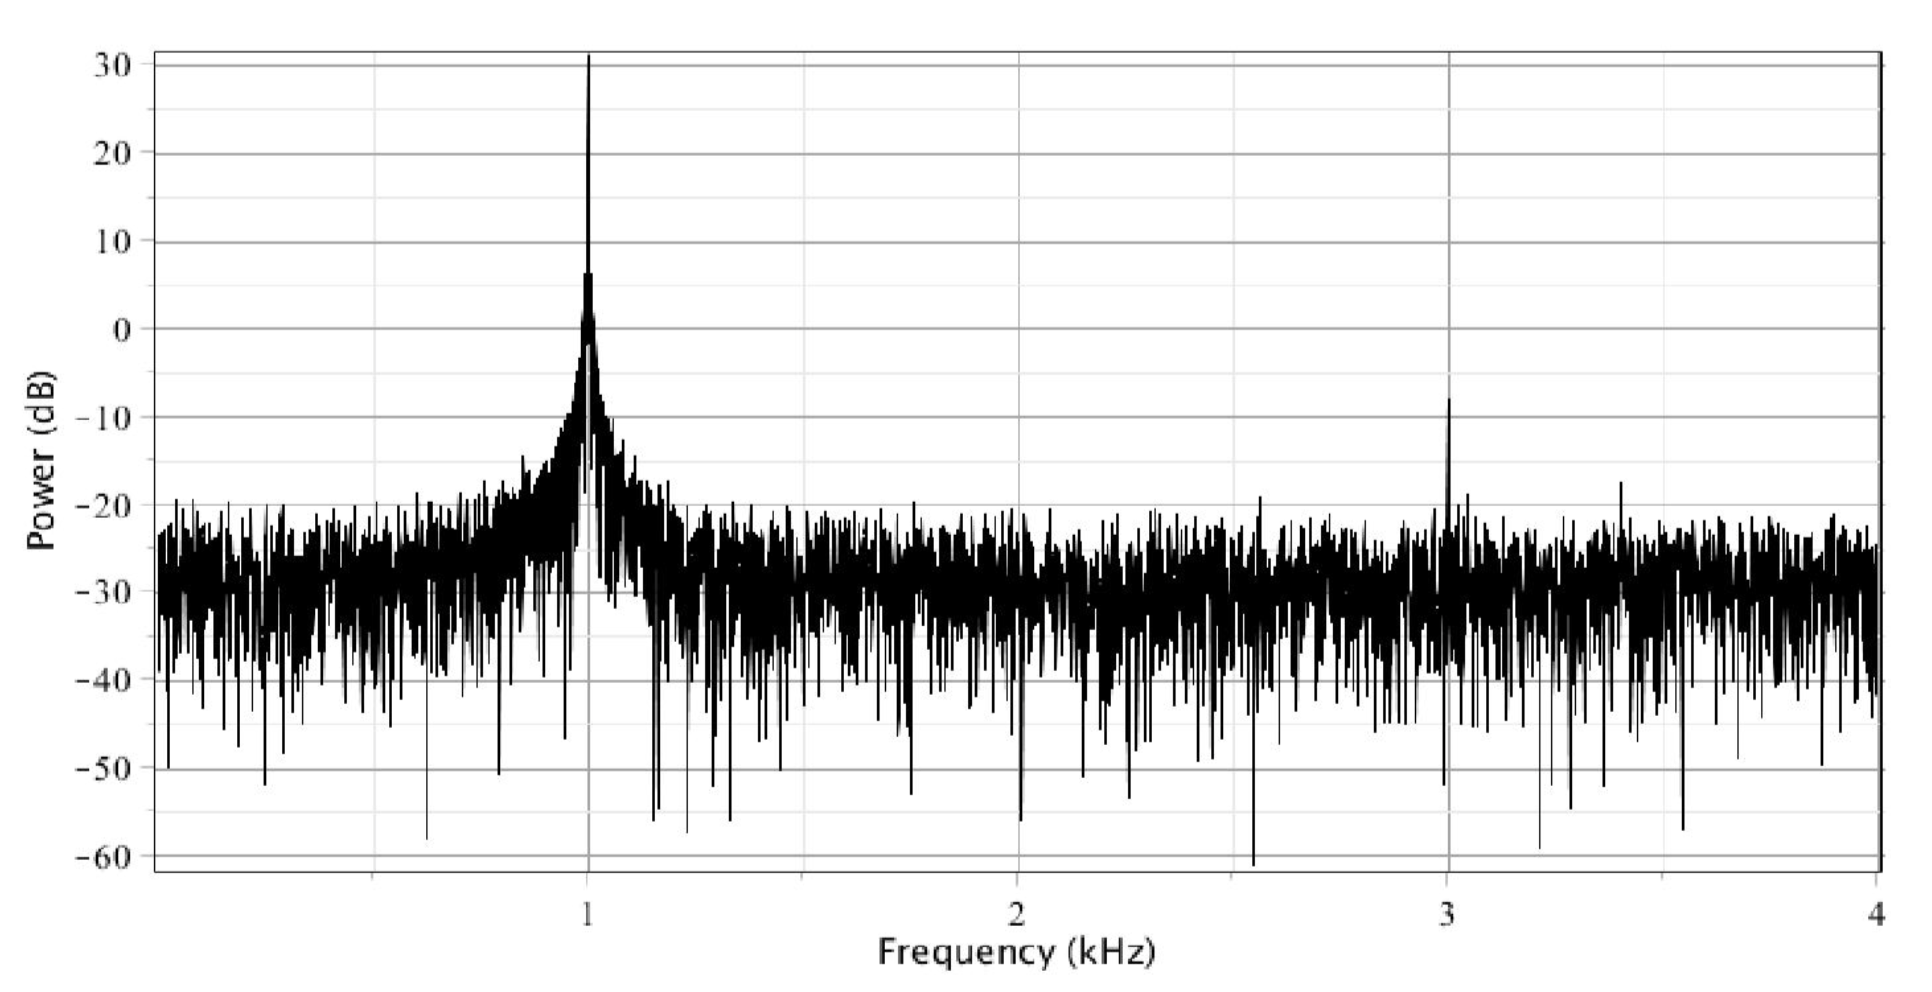
\includegraphics[width=\linewidth]{img/1khz_power}
  \caption{Frequenzspektrum ($ \left| \hat{s}(2 \pi f) \right| $) eines 1kHz-Signals mit Störgeräuschen. Der Leistungspegel stellt hierbei eine logarithmische Skalierung dar. Quelle: (\url{ http://www.maplesoft.com/products/maple/features/Signal_Processing.aspx},  21.11.15)}
  \label{img:1khz_power}
\end{figure}

\subsection{Spektrogramm}
Insbesondere bei der Analyse von Musikinstrumenten ist nicht nur die Frequenzverteilung des ganzen Signals wichtig, sondern auch deren zeitlicher Verlauf. Indem man das Signal in kleinere Untereinheiten teilt (Die Anzahl der Messwerte pro Paket ist aus technischen Gründen für die FFT meist eine Potenz zur Basis 2) und einzeln analysiert. Diese Kaskade aus Freuqenzspektren lässt sich in einem Spektrogramm darstellen, indem auf der y-Achse die Frequenz udn auf der x-Achse der Zeitraum der Fouriertransformation aufgetragen wird. Die Amplitude wird durch, von Quelle zu Quelle unterschiedlichen, Farbverläufen dargestellt.

Für die Spektrogramme ergiebt sich immer eine Unschärfe zwischen Frequenz und Zeit. Je mehr Messpunkte für die einzelne Transformation herangezogen werden, desto höher ist die Frequenzauflösung. Die entstehende Transformation ist jedoch nicht mehr aussagekräftig für Momentaufnahmen der Zeit.
